\section{实验步骤}

本章节将介绍本次实验的步骤,包括实现特征点距离计算的函数,实现特征点匹配的函数,运行测试脚本。

\subsection{实现特征点距离计算的函数}

根据上述介绍,特征点距离的计算可以通过欧式距离、余弦距离等方式来实现。

\begin{lstlisting}[style=Python]
def compute_feature_distances(features1, features2):
    mode = 'euclidean'
    if mode == 'euclidean':
        return np.sqrt(np.sum((features1[:, None] - features2) ** 2, axis=2))
    if mode == 'manhattan':
        return np.sum(np.abs(features1[:, None] - features2), axis=2)
    if mode == 'chebyshev':
        return np.max(np.abs(features1[:, None] - features2), axis=2)
    if mode == 'minowski':
        p = 3
        return np.sum(np.abs(features1[:, None] - features2) ** p, axis=2) ** (1 / p)
\end{lstlisting}

完整的代码请参见附录\ref{appendix:code}。上述代码实现了4种距离的计算方式,包括欧式距离、曼哈顿距离、切比雪夫距离和闵可夫斯基距离。通过调整\texttt{mode}参数,可以选择不同的距离计算方式。

不同的距离度量方式具有不同的特点,例如欧式距离是最常见的距离计算方式,但是随着维度的增大,其度量也越困难;曼哈顿距离是在欧式距离的基础上,将距离的平方换成了距离的绝对值,因此更适合于计算城市街道的距离;切比雪夫距离是在欧式距离的基础上,取各个坐标距离的最大值,其适用范围非常特殊;闵可夫斯基距离是以上三种距离的推广,可以通过调整参数$p$来实现不同的距离计算方式。

\subsection{实现特征点匹配的函数}

在实现距离计算的函数之后,我们可以通过比较两个特征点的距离来进行特征点的匹配。

\begin{lstlisting}[style=Python]
def match_features(features1, features2, x1, y1, x2, y2):
    def mean_distance_filter(dists, alpha):
        mean_dist = np.mean(dists)
        std_dist = np.std(dists)
        return dists < mean_dist - alpha * std_dist
    
    def mean_cosine_filter(cosines, alpha):
        mean_cosine = np.mean(cosines)
        std_cosine = np.std(cosines)
        return cosines > mean_cosine + alpha * std_cosine
    
    def dist_ratio_filter(best_match_dists, second_match_dists, thresh):
        return (best_match_dists / second_match_dists) < thresh
    
    def cross_validation_filter(best_matches, inv_best_matches):
        return inv_best_matches[best_matches] == np.arange(best_matches.shape[0])
    
    def spatial_filter(shifts, cosine_thresh, dist_thresh):
        mean_direction = np.mean(shifts, axis=0, keepdims=True)
        cosine = np.sum(shifts * mean_direction, axis=1) / (np.linalg.norm(shifts, axis=1) * np.linalg.norm(mean_direction, axis=1))
        cosine_mask = cosine > cosine_thresh
        dists = np.linalg.norm(shifts, axis=1)

        mean_dist = np.mean(dists)
        std_dist = np.std(dists)
        dist_mask = (dists > mean_dist - dist_thresh * std_dist) & (dists < mean_dist + dist_thresh * std_dist)

        return cosine_mask & dist_mask
    
    mode = 'euclidean'
    dist_alpha = 0.1
    cosine_alpha = 0.7
    ratio_thresh = 0.8
    spatial_cosine_thresh = 0.6
    spatial_dist_thresh = 1.0
    
    dists = compute_feature_distances(features1, features2)
    cosines = np.dot(features1, features2.T) / (np.linalg.norm(features1) * np.linalg.norm(features2))
    best_matches = np.argmin(dists, axis=1)
    inv_best_matches = np.argmin(dists, axis=0)
    best_match_dists = dists[np.arange(dists.shape[0]), best_matches]
    second_match_dists = dists[np.arange(dists.shape[0]), np.argsort(dists, axis=1)[:, 1]]
    best_match_cosines = cosines[np.arange(cosines.shape[0]), best_matches]

    ...

    dist_mask = mean_distance_filter(best_match_dists, dist_alpha)
    cosine_mask = mean_cosine_filter(best_match_cosines, cosine_alpha)
    ratio_mask = dist_ratio_filter(best_match_dists, second_match_dists, ratio_thresh)
    cross_val_mask = cross_validation_filter(best_matches, inv_best_matches)
    mask = dist_mask & cosine_mask & ratio_mask & cross_val_mask
    inds1, inds2 = np.arange(features1.shape[0]), best_matches
    matches = np.stack([inds1[mask], inds2[mask]], axis=1)
    confidences = 1 / best_match_dists[mask]

    x1, y1 = x1[matches[:, 0]], y1[matches[:, 0]]
    x2, y2 = x2[matches[:, 1]], y2[matches[:, 1]]
    shifts_x = x1 - x2
    shifts_y = y1 - y2
    shifts = np.stack([shifts_x, shifts_y], axis=1)
    spatial_mask = spatial_filter(shifts, spatial_cosine_thresh, spatial_dist_thresh)

    matches = matches[spatial_mask]
    confidences = confidences[spatial_mask]
    return matches, confidences
\end{lstlisting}

完整的代码请参见附录\ref{appendix:code}。上述代码实现了特征点匹配的函数,通过调整不同的参数,可以实现不同的特征点匹配方式。

具体来说,上述代码实现计算特征点之间的距离,之后通过一系列的过滤器来筛选出最终的匹配结果。这些过滤器包括距离过滤器、余弦相似度过滤器、距离比例过滤器、交叉验证过滤器和空间过滤器。下面将逐一介绍这些过滤器:

\begin{itemize}
    \item 距离过滤器:通过计算特征点之间的距离$d$,然后计算距离的均值$\mu$和标准差$\sigma$,之后根据准则$d < \mu - \alpha \sigma$来筛选出距离较小的特征点。
    \item 余弦相似度过滤器:通过计算特征点之间的余弦相似度$s$,然后计算余弦相似度的均值$\mu$和标准差$\sigma$,之后根据准则$s > \mu + \alpha \sigma$来筛选出余弦相似度较大的特征点。
    \item 距离比例过滤器:通过计算到最近邻特征点的距离$d_1$和次近邻特征点之间的距离$d_2$,然后根据准则${d_1}/{d_2} < \text{thresh}$来筛选出符合距离比例的特征点。
    \item 交叉验证过滤器:首先计算集合$A$中的特征点到集合$B$中的特征点的最近邻,然后计算集合$B$中的特征点到集合$A$中的特征点的最近邻,之后仅保留两个集合中的特征点相互为最近邻的特征点。
    \item 空间过滤器:通过计算特征点在空间上的偏移量,然后计算偏移量的均值$\mu$和标准差$\sigma$,之后提出2种准则,分别是偏移量$\vec{\delta}$与平均偏移量$\overline{\vec{\delta}}$的余弦相似度大于阈值,以及偏移量的长度$d$与平均长度$\overline{d}$的差值在一定范围内。即$\cos(\vec{\delta}, \overline{\vec{\delta}}) > \tau$和$\mu - \gamma \sigma < d < \mu + \gamma \sigma$。
\end{itemize}

之所以这些过滤器有效,是因为它们可以通过一定的准则来筛选出符合特定条件的特征点。例如,距离和余弦相似度过滤器考虑到理想的匹配往往具有较小的距离和较大的余弦相似度,因此通过这两个准则可以筛选出较好的匹配结果。

距离比例过滤器是SIFT算法中的一个重要步骤,通过计算最近邻和次近邻之间的距离比例,可以筛选出较好的匹配结果。可以想象,如果某个特征点同时与多个特征点距离相近,那么这个特征点可能是一个较差的匹配结果。因此,通过距离比例过滤器可以排除这种情况。

交叉验证过滤器是为了排除特征点之间的多对多匹配。例如,如果特征点$A$是特征点$B$的最近邻,那么特征点$B$也应该是特征点$A$的最近邻。通过这种方式,可以排除多对多匹配的情况。

空间过滤器是从空间的角度来考虑特征点的匹配。通过计算特征点之间的偏移量,然后计算偏移量的均值和标准差,可以得到特征点之间的平均偏移量。由于特征点之间的偏移量应该是比较稳定的,因此通过这种方式可以排除一些不稳定的匹配结果。

通过上述步骤,可以得到最终的匹配结果。下一步将介绍如何运行测试脚本。

\subsection{运行测试脚本}

在实现了特征点距离计算的函数和特征点匹配的函数之后,我们可以通过运行测试脚本来测试这些函数。在命令行中执行如下命令:

\begin{lstlisting}[language=Bash]
jupyter notebook
\end{lstlisting}

然后在浏览器中打开\texttt{http://localhost:8888},如图\ref{fig:jupyter}所示,找到对应的测试脚本,点击运行即可。

\begin{figure}[H]
    \centering
    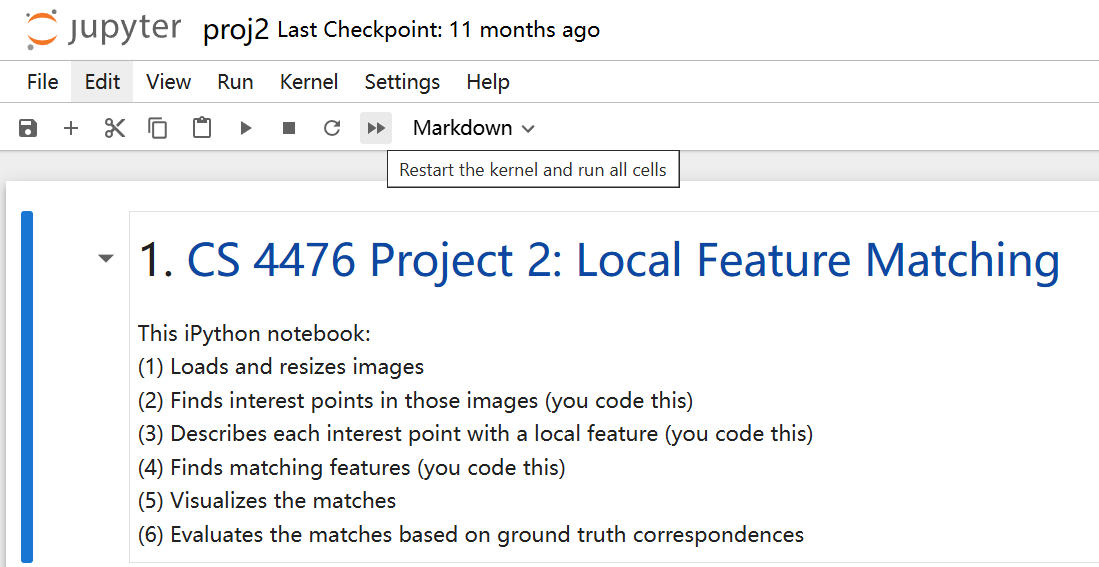
\includegraphics[width=0.8\textwidth]{images/jupyter.png}
    \caption{Jupyter Notebook界面}
    \label{fig:jupyter}
\end{figure}

如图\ref{fig:correct}所示,所有结果均通过验证。

\begin{figure}[H]
    \centering
    \begin{minipage}[b]{0.45\linewidth}
        \subfloat [] {
            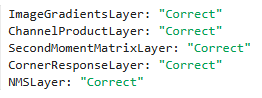
\includegraphics[width=\textwidth]{images/correct1.png}
        }
        \\
        \subfloat [] {
            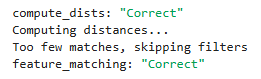
\includegraphics[width=\textwidth]{images/correct3.png}
        }
    \end{minipage}
    \begin{minipage}[b]{0.45\linewidth}
        \subfloat [] {
            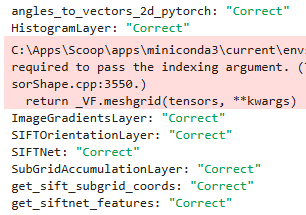
\includegraphics[width=\textwidth]{images/correct2.png}
        } 
    \end{minipage}
    \caption{Jupyter Notebook运行结果}
    \label{fig:correct}
\end{figure}